\documentclass[conference]{IEEEtran}
\IEEEoverridecommandlockouts
\usepackage{cite}
\usepackage{amsmath,amssymb}
\usepackage{graphicx}
\usepackage{array}
\usepackage{booktabs}
\usepackage{xcolor}
\usepackage{url}
\usepackage[hidelinks]{hyperref}
\graphicspath{{../docs/figures/}}
% Tighter, less stretchable space between floats and text (IEEEtran default is 1.7\baselineskip).
\setlength{\textfloatsep}{10pt plus 2pt minus 2pt}
\setlength{\floatsep}{8pt plus 2pt minus 2pt}
\setlength{\dbltextfloatsep}{10pt plus 2pt minus 2pt}
% Bold section headings (IEEEtran conference default, plus \bfseries).
\makeatletter
\def\section{\@startsection{section}{1}{\z@}{1.5ex plus 1.5ex minus 0.5ex}%
{0.7ex plus 1ex minus 0ex}{\normalfont\normalsize\centering\scshape\bfseries}}%
\makeatother
% Leave spare space at the column foot instead of stretching it between paragraphs.
\raggedbottom
% Visible marker for anything still to be checked; must be empty before submission.
\newcommand{\todo}[1]{\textcolor{red}{[TODO: #1]}}

\begin{document}

\title{What Benchmark Scores Hide: Auditing a Flow-Based IoT Intrusion Detector from Labels to Live Blocking}

\author{\IEEEauthorblockN{Muhammad Usama}
\IEEEauthorblockA{Department of Computer Science\\
COMSATS University Islamabad, Pakistan\\
sp23-bcs-069@isbstudent.comsats.edu.pk}
\and
\IEEEauthorblockN{Ahmad Kamran Malik}
\IEEEauthorblockA{Department of Computer Science\\
COMSATS University Islamabad, Pakistan\\
ahmad.kamran@comsats.edu.pk}}

% Trim IEEEtran's default gap between the author block and the abstract.
\IEEEaftertitletext{\vspace{-1.5\baselineskip}}
\maketitle

\begin{abstract}
Benchmark scores for network intrusion detectors hide problems that appear in deployment. We audit a decision tree on 54 NFStream flow features from labels to live blocking on an emulated Open vSwitch gateway, and condense the audit into four checks. \emph{Labels:} background, i.e.\ traffic outside the attack, makes up 90.9--98.5\% of the flows in six of the nine CIC-IoT2023 attack captures. Trained on file-name labels, the tree flags 71--88\% of the background flows in unseen attack captures, against 0.5--5.4\% with evidence labels; on IoT-23 it flags 23--47\% of unseen benign devices' flows, against 0--17.5\% with the authors' Zeek labels. \emph{Splits:} on CIC-IoT2023 a random split hides that brute-force recall falls from 1.00 to 0.05 when the attack moves from SSH passwords to RTSP stream paths; this case (three host pairs) is most of the random--temporal gap. On IoT-23 the gap comes from classes missing from one split half. \emph{Live:} matching live to offline flows one by one exposed a forwarding pitfall, idle flow meters, an NFStream export-ordering defect (median verdict delay 82.5\,s) and flow splitting at slow replay under unchanged macro-F1. \emph{Response:} blocking a host pair on its first attack verdict caused 60 false blocks in ten minutes; requiring 10 verdicts caused none in the ten live windows (3 in 5.9\,h with persistent counters) but missed the Mirai bots and the web attackers. Timed at flow export, verdicts let 11\% of attack flows start after their block, not 97\%. Code and results are public.

\end{abstract}

\begin{IEEEkeywords}
intrusion detection, Internet of Things, evaluation methodology, dataset labeling, flow export, CIC-IoT2023
\end{IEEEkeywords}

\section{Introduction}\label{sec:intro}

Machine-learning network intrusion detection systems (NIDS) are mostly evaluated on public benchmarks, where reported scores are often near the maximum. Such scores say little about an IoT gateway, which has a few CPU cores, sees traffic in time order, builds flows itself and must act on its verdicts; operators, too, act on aggregated reports, not on single samples a classifier flagged~\cite{apruzzese2026reshaping}. The gap between benchmark and operation is long known~\cite{sommer2010outside} and well documented for security machine learning~\cite{arp2022dos,apruzzese2023sok}; a recent study reports a random forest with hold-out F1 0.97 on UNSW-NB15 that detected 1 of 105 attacks (recall 0.0095) in operational validation on a small labeled laboratory capture~\cite{tang2026hybrid}.

\begin{table}[t]
\centering
\caption{The four-check audit and what it caught. Checks~1--2 were run on CIC-IoT2023 and IoT-23, Checks~3--4 on CIC-IoT2023. FPR: Benign false-positive rate; host pair: unordered address pair within one capture.}
\label{tab:checklist}
\footnotesize
\setlength{\tabcolsep}{3pt}
\begin{tabular}{>{\raggedright\arraybackslash}p{1.55cm}>{\raggedright\arraybackslash}p{3.2cm}>{\raggedright\arraybackslash}p{3.25cm}}
\toprule
Check & Measure & Caught here \\
\midrule
1 Labels & Background share per capture; FPR of a file-label tree on captures it never saw & 71--88\% of unseen CIC-IoT2023 background flagged (0.5--5.4\% with evidence labels); released CSVs allow only file-name labels \\
\addlinespace[2pt]
2 Splits & Per-class temporal recall with host-pair counts; class presence in both halves; cluster-unit sensitivity; boundary-spanning share & Brute-force target change on 3 host pairs (CIC-IoT2023); gap from missing classes, not robust to the cluster unit (IoT-23) \\
\addlinespace[2pt]
3 Live & Flow-by-flow match on every run; packet accounting; replay rate; delay vs.\ CPU budget & Forwarding pitfall, idle meters, export-ordering defect; flows split at slow replay \\
\addlinespace[2pt]
4 Response & False blocks per host-pair window; trade-off over $k$ per class and counter horizon & 60 false blocks in 10\,min at $k=1$, none at $k=10$; Mirai missed by the flow-count rule; 11\% of attack flows start after their block, 97\% offline \\
\bottomrule
\end{tabular}
\end{table}

Each source of this gap is known on its own: label errors in benchmarks~\cite{engelen2021troubleshooting,liu2022error,lanvin2023errors,flood2024smells}, splits that ignore time~\cite{pendlebury2019tesseract,arp2022dos,andresini2021insomnia}, exporters and timeouts that change the flows~\cite{velan2020impact,pinto2025flowexporter}, and detectors that fall short once traffic arrives as a stream~\cite{pekar2025early,zhao2026gidseval}. We do not claim a new failure mode, and we propose no new detection method. Instead we follow one ordinary detector along the whole path: a decision tree over 54 NFStream~\cite{aouini2022nfstream} flow statistics, trained on ten captures of CIC-IoT2023~\cite{neto2023ciciot2023}, with the label and split stages repeated on ten IoT-23 captures~\cite{garcia2020iot23}. At each of four stages (labels, splits, live gateway, response) we ask what a standard evaluation would hide and which check reveals it. The checks share one move: each replaces an aggregate score with the unit at which the problem shows, namely the capture (labels), the host pair (splits), the individual flow (live) and the host-pair window (response). The contributions are:
\begin{itemize}
\item \emph{A four-check audit} (Table~\ref{tab:checklist}), released as scripts. Checks~1 and~2 apply known pitfalls~\cite{arp2022dos,flood2024smells} per capture and host pair; Checks~3 (live/offline flow fidelity) and~4 (false blocks) go beyond offline evaluation.
\item \emph{Labels} (Section~\ref{sec:labels}): to our knowledge the first per-capture background share for CIC-IoT2023 (90.9--98.5\% in six of the nine attack captures), and its cost on captures the model never saw, on two datasets, one of them with the dataset authors' labels.
\item \emph{Splits} (Section~\ref{sec:splits}): a decomposition showing that 78\% of a $+0.14$ random--temporal macro-F1 gap on CIC-IoT2023 is one class changing its attack target on three host pairs, while on IoT-23 the gap comes from classes missing from one half of the split; flow-level confidence intervals are several times too narrow.
\item \emph{Live fidelity} (Section~\ref{sec:live}): a flow-by-flow live/offline match that exposed a previously undiagnosed cause of late flow export in NFStream, invisible offline (nfstream\#262~\cite{nfstream262}; fix submitted as PR~\#263~\cite{nfstream263}), and flow splitting that macro-F1 did not show.
\item \emph{Response} (Section~\ref{sec:response}): false blocks per host-pair window over the number $k$ of verdicts required per host pair, and what export delay does to prevention in 60\,s windows: 97\% of attack flows start after their pair is blocked when verdicts are stamped at flow end, as an offline evaluation does, but 11\% once the 15\,s idle timeout delays them.
\end{itemize}

\section{Related Work}\label{sec:related}

\emph{Labels.} Label and flow-construction errors in NIDS benchmarks are well documented for CIC-IDS2017 and CSE-CIC-IDS2018~\cite{engelen2021troubleshooting,liu2022error}, and correcting them changes detection scores~\cite{lanvin2023errors}. Flood et al.\ catalog design smells of benchmark datasets~\cite{flood2024smells}, and models trained on such benchmarks can rely on shortcuts rather than attack behavior~\cite{jacobs2022emperor}. Of 36 network security datasets analyzed by Garcia and Valeros, 11 label flows, while file or directory names combined (14) are more common than any other style~\cite{garcia2023labeling}. For CIC-IoT2023~\cite{neto2023ciciot2023}, Ramkumar et al.\ observed that the captures mix benign and attack traffic and re-filtered them per device by MAC address, but did not quantify the mixing~\cite{ramkumar2024diagnosing}; Vitorino et al.\ re-extract CIC-IoT2023 flows and assume that each capture contains only its named attack~\cite{vitorino2025revisiting}. Kostas et al.\ note that the attack pcaps of IoT-NID also contain benign packets, and that the derived IoTID20 flows label all of them as attacks~\cite[App.~A.3]{kostas2024iotgem}. Background traffic in attack captures is therefore not new; we add its share per capture for CIC-IoT2023 and the cost of file-name labels on captures the model never saw.

\emph{Splits.} Random splits of time-ordered data are a known pitfall in security machine learning~\cite{arp2022dos,pendlebury2019tesseract,apruzzese2023sok}, time-aware evaluation has been applied to NIDS~\cite{andresini2021insomnia}, and tree classifiers degrade over time on MAWI flows~\cite{schraven2026mawiflow}. On IoT-23, Lyon et al.\ train on earlier months and find performance degrading as new malware types appear~\cite{lyon2026iot23drift}. In a time-shift experiment, Traffic-MoE uses a chronological split (first 40\% of the time span for training, last 40\% for testing, the middle 20\% discarded as a buffer) on CIC-IoT2023 and CICIoMT2024, using byte-level flow tokens~\cite{zhou2026trafficmoe}; BRIDGE uses an early/late split in a pooled benchmark~\cite{bridge2026tchnet}; and Rasheed and Alobaedy find that drift causes no consistent decrease in performance but ``specific behavior changes, such as total blindness, sensitivity inflation and relatively stable detection''~\cite{rasheed2026drift}. IoTGeM trains on telnet and tests on RTSP brute force, by design, and finds that the variants do not generalize~\cite{kostas2024iotgem}. Our split, within each capture, has no buffer; we measure the connections that span it and trace the gap per class and host pair.

\emph{Live detection and exporters.} Learned detectors on IoT gateways are common~\cite{realguard2022}, as are Mininet/Open vSwitch (OVS)~\cite{lantz2010mininet,pfaff2015ovs} prototypes that block flagged hosts. Export timeouts delay flow-based detection~\cite{hofstede2013realtime}, the choice of expiration timeouts changes the flow records and can severely affect detection~\cite{velan2020impact}, and the exporter changes detection results~\cite{pinto2025flowexporter,pinto2025hera} and what a model sees~\cite{vitorino2025revisiting}. Models trained on complete flows lose up to 30\% precision and recall, under certain conditions, when tested on partial flows~\cite{pekar2025early}, and a streaming replay of graph-based NIDS found that none of 18 detector--dataset pairs could alert as events arrive~\cite{zhao2026gidseval}. We add a check that a live gateway classifies the flows of the offline evaluation.

\emph{Response.} Blocking via OpenFlow/OVS drop rules is standard in software-defined networking (SDN) DDoS mitigation~\cite{bawany2017ddos,yan2016sdn}, and a recent SoK reviews how machine-learning SDN defenses are evaluated~\cite{orsdemir2026sok}. Apruzzese argues that NIDS research should evaluate in real, even synthetic, networks and account for how operators act on reports~\cite{apruzzese2026reshaping}. Few works we found report how many benign hosts a blocking policy cuts off on replayed traffic.

\section{Detector and Evaluation Setup}\label{sec:setup}

\emph{CIC-IoT2023.} We use ten captures~\cite{neto2023ciciot2023}: Benign, DDoS-SYN, DoS-HTTP, Recon-PortScan, MITM-ArpSpoofing, DictionaryBruteForce, SqlInjection, XSS, CommandInjection and Mirai-udpplain (about 5.17\,GB). Files over 300\,MB are trimmed to their first $10^6$ packets. The captures map to eight classes: Benign, BruteForce, DDoS-SYN, DoS-HTTP, MITM-ARP (man-in-the-middle by ARP spoofing), Mirai, Recon and Web (SQL injection, XSS and command injection).

\emph{IoT-23.} We use ten IoT-23 captures~\cite{garcia2020iot23}: seven malware captures (Hide\&Seek, Muhstik, Hakai, two Torii, Mirai, Trojan) and three captures of real, uninfected IoT devices (Philips Hue bridge, Amazon Echo, Somfy smart door lock; of 7-1 only its Somfy-01 part), which we call benign-device captures. The Okiru captures (all at least 1\,GB) are left out. Labels are the dataset's own Zeek \texttt{conn.log.labeled}: each flow is joined to the Zeek connection with the same unordered 5-tuple and the nearest start within $\pm2$\,s, otherwise to the Zeek connection whose span contains the flow's start. Over 99.99\% of the 756,306 flows match; the rest are dropped, and only 0.04\% overlap Zeek rows of more than one class. The six classes are Benign, PortScan, C\&C, Attack (only in capture 3-1), DDoS and FileDownload.

\emph{Flows and features.} We build flows with NFStream~\cite{aouini2022nfstream} (version 6.6.0), using its statistical features, an idle timeout of 15\,s and an active timeout of 120\,s, with identical settings for both datasets and on the live gateway. The model uses 54 statistical features (packet counts and sizes, inter-arrival times, durations, TCP flag counts per direction). Identifiers (addresses, ports, protocol, timestamps) are excluded, because they let a model memorize the capture~\cite{arp2022dos}. CIC-IoT2023 yields 857,206 labeled flows, 511,527 of them DDoS-SYN (a consequence of trimming).

\emph{Detector.} The detector is a scikit-learn~\cite{pedregosa2011sklearn} decision tree with balanced class weights. Limiting depth and leaf size raised the validation Benign FPR, so the \emph{deployed tree} (depth 32; 1,767 nodes, 222\,KiB) is effectively unconstrained. On the CIC-IoT2023 temporal split it scores macro-F1 0.725 (Benign FPR 3.8\%), close to a random forest (0.737, at about 94$\times$ the size and 63$\times$ the single-flow latency) and histogram gradient boosting (0.714). NSGA-II feature selection~\cite{deb2002nsga2,blank2020pymoo} kept 14 of 54 features at no measurable cost but barely shrank the tree. All results use the deployed tree, retrained with the same settings for each dataset and label set (except the check of the released CSVs in Section~\ref{sec:labels}).

\emph{Splits.} The \emph{temporal} split puts the first 70\% of each capture's flows, by start time, into training (on CIC-IoT2023, 600,050 training and 257,156 test flows). The \emph{random} split draws 70\% at random, stratified by class. Every design choice (tree limits, feature subset, blocking policy) is made on a validation set, the last 20\% of each capture's training period.

\emph{Metrics.} We report per-class F1 and recall with test support, macro-F1 over all classes, and the Benign false-positive rate (FPR), the share of Benign test flows predicted as any attack. A \emph{host pair} is an unordered pair of addresses within one capture. Flows from one host pair are not independent, so 95\% confidence intervals (CIs) come from a \emph{host-pair bootstrap}: 1,000 resamples of whole host pairs. A flow-level bootstrap~\cite{efron1994bootstrap} gives far too narrow intervals: [0.702, 0.741] for the temporal macro-F1, against [0.568, 0.822] with host pairs. Two splits are compared by a \emph{paired} bootstrap over the union of both test sets' host pairs: each resample draws host pairs with replacement and applies the same draw to both splits (a pair absent from one test set adds nothing to it).

\section{Check 1: Labels}\label{sec:labels}

\emph{What the benchmark hides.} Each CIC-IoT2023 capture is named after one attack, and all its flows are commonly labeled with that name; but the captures were recorded on a network of active IoT devices, so the attack is only part of the traffic. We call the Benign flows inside an attack capture \emph{background}. Garcia and Valeros predict that models trained with one label per PCAP ``may learn to detect operating system benign traffic as malicious'' (Sec.~3.2)~\cite{garcia2023labeling}; we measure this on traffic the model never saw.

\emph{Evidence labels.} We identified the attackers and victims in every attack capture from the packets themselves (Table~\ref{tab:background}): HTTP payloads against the DVWA (Damn Vulnerable Web Application) test site for the web attacks, destination ports and their timing for brute force, top talkers for the floods, Mirai and the port scan, and ARP replies for MITM-ARP. A flow is labeled as an attack only if (i) one endpoint is a confirmed attacker and the other a victim, on the attack's port where known, or (ii) for ARP spoofing, its first packet was sent from or to the attacker's MAC address and the attacker's own IP is not an endpoint, i.e.\ it is a victim's traffic relayed through the attacker. Every other flow is Benign.

\begin{table}[t]
\centering
\caption{Background share (Benign flows under evidence labels) of each attack capture, and the evidence that confirmed the attacker. Addresses are last octets in 192.168.137.0/24.}
\label{tab:background}
\footnotesize
\setlength{\tabcolsep}{3pt}
\begin{tabular}{lrr>{\raggedright\arraybackslash}p{3.85cm}}
\toprule
Capture & Flows & Backgr. & Attacker evidence \\
\midrule
XSS          &   4,992 & 98.5\% & \texttt{<script>} from .147 \\
CmdInj       &   5,639 & 98.3\% & DVWA \texttt{exec} page from .147 \\
MITM-ARP     &  12,208 & 97.6\% & MAC \ldots:27:d5 claims .1 and .65 \\
SQLi         &   7,383 & 94.8\% & \texttt{SLEEP(5)}, \texttt{UNION SELECT} \\
Mirai        &     653 & 93.7\% & 7 bots to .191 (UDP) \\
BruteForce   &  11,824 & 90.9\% & .65 to SSH :22, then RTSP :554 \\
Recon        & 205,065 & 30.2\% & .178: 1,001 ports on 58 hosts \\
DoS-HTTP     &  51,275 & 23.0\% & .66 to .71/.141:80 \\
DDoS-SYN     & 511,936 &  0.1\% & 6 sources to .245:4070 \\
\bottomrule
\end{tabular}
\end{table}

\emph{Background share.} Background makes up 90.9--98.5\% of the flows in six of the nine attack captures (web, brute force, MITM-ARP, Mirai) (Table~\ref{tab:background}); overall, file-name and evidence labels differ for 13.4\% of the 857,206 flows.

\emph{The cost of file-name labels on unseen traffic.} We trained the same tree on file-name labels and on evidence labels and measured the Benign FPR. Within a split this is partly circular: the file-label tree is tested on the later background of captures whose earlier background it learned under the capture's name. We therefore also train on nine captures and test on the tenth (leave one capture out, LOCO; Table~\ref{tab:filelabel}). On a held-out attack capture, the file-label tree flags 71--88\% of the background flows, against 0.5--5.4\% for the tree trained on evidence labels, and more in each of the nine captures. (Holding out the single Benign capture leaves the file-label tree no Benign training flow.) Within the temporal split, most of its false positives (89\%) are background inside attack captures. Scored against file-name labels, the two trees swap places, because correct Benign verdicts in attack captures then count as misses. The random split gives the same pattern.

\begin{table}[t]
\centering
\caption{The tree trained on file-name labels (file) or on evidence (CIC-IoT2023) or Zeek (IoT-23) labels. Macro-F1 scored against file-name labels (as a file-label study would report) or against evidence/Zeek labels. Benign FPR on background in attack captures and on the benign capture(s). LOCO: range over held-out captures. CIC: CIC-IoT2023. --: not computed. Original labels (corrected values in the text). The two IoT-23 values 0.649 are 0.6486 (file) and 0.6487 (Zeek).}
\label{tab:filelabel}
\footnotesize
\setlength{\tabcolsep}{2.6pt}
\begin{tabular}{lllcccc}
\toprule
 & & Trained & \multicolumn{2}{c}{Macro-F1 vs.} & \multicolumn{2}{c}{Benign FPR} \\
\cmidrule(lr){4-5}\cmidrule(lr){6-7}
Data & Test & on & file & evid./Zeek & backgr. & benign capt. \\
\midrule
CIC & temporal & file  & 0.537 & 0.396 & 86.1\% & 31.4\% \\
            & temporal & evid. & 0.409 & 0.725 & 4.8\% & 1.0\% \\
            & LOCO     & file  & --    & --    & 71.4--87.8\% & (100\%) \\
            & LOCO     & evid. & --    & --    & 0.5--5.4\% & 1.5\% \\
\midrule
IoT-23      & temporal & file  & 0.649 & 0.169 & 99.97\% & 4.7\% \\
            & temporal & Zeek  & 0.157 & 0.649 & 3.4\% & 0.18\% \\
            & LOCO     & file  & --    & --    & 9.4--99.95\% & 23.4--46.7\% \\
            & LOCO     & Zeek  & --    & --    & 0--49.1\% & 0--17.5\% \\
\bottomrule
\end{tabular}
\end{table}

\emph{Label audit.} Our first DDoS-SYN labeling missed a sixth source (.36) that joins after the first 300,000 packets; error analysis found it as 65,525 ``Benign'' flows predicted as DDoS-SYN, and we re-checked every flood victim over the whole trimmed file. Because this revision moved labels towards the model, we then audited the labels blind and in both directions. A fixed program rated 975 test flows, sampled per capture, label and model agreement, from their own packets, without seeing the label, the attacker list or the verdict; defects of the rater found in its first run were fixed (Section~\ref{sec:threats}). Of the 630 flows it could decide, 2 of 265 attack labels were wrong (UPnP requests of the SQLi attacker to a non-victim) and 22 of 365 Benign labels, all from the DoS-HTTP attacker flooding a third server (.174) missing from our victim list. Weighted by stratum size, this puts 4.3\% of the Benign-labeled test flows (the whole flood) and almost none of the attack-labeled ones in error. With at most 30 flows per stratum, a stratum without a found error can still hold up to 11--13\% errors, and the undecided flows, mostly short or without payload, lie mainly where label and model disagree; errors there cannot be ruled out. MITM-ARP is rated by the MAC relay that defines its label, so for it the audit checks only consistency. The abstract and tables keep the original labels, which understate the evidence-label tree: with both errors corrected, its Benign FPR is 1.3\% instead of 3.8\% and its macro-F1 0.729 instead of 0.725; file-label numbers move by at most 1.3 points.

\emph{Robustness test on IoT-23.} IoT-23 tests the result against labels that are not ours (the authors' Zeek labels). For file-name labels we map each malware family to its main behavior, e.g.\ Hide\&Seek to PortScan, Torii to C\&C and Mirai to DDoS; this mapping is our choice. The background share (Zeek label Benign) of the malware captures ranges from 5.5\% to 99.9\%. The benign-device captures are the out-of-capture test (Table~\ref{tab:filelabel}): under LOCO the file-label tree flags more of a held-out benign device's flows than the Zeek-label tree in each of the three captures. Generalization to an unseen capture is hard regardless of labels: the Zeek-label tree also flags 42--49\% of the background in two held-out malware captures. In-capture, the file-label tree flags nearly all background in every malware capture, which mainly shows that it learned each capture's name.

\emph{The benchmark as distributed.} Every study that uses the released CSVs inherits file-name labels. The CSVs (mirror \texttt{bencorn/CIC-IoT-2023}) hold 39 packet-window features without address or timestamp, labeled only by the file name, with rows shuffled, so they cannot be relabeled from evidence. Even scored against file-name labels on a random split, a decision tree and a random forest on these CSVs reach macro-F1 0.75--0.80 but recall below 0.45 on BruteForce and Web, so the weak low-rate classes are not an artifact of our NFStream flows.

\section{Check 2: Splits}\label{sec:splits}

\emph{What a random split hides.} Table~\ref{tab:perclass} gives per-class results on CIC-IoT2023. Macro-F1 is 0.867 under the random split (host-pair CI [0.733, 0.875]) and 0.725 ([0.568, 0.822]) under the temporal split. The paired bootstrap puts the difference (random minus temporal) at +0.142 [0.025, 0.287], but almost all of it is one class: BruteForce contributes 78\% of the summed per-class F1 difference. These intervals score a class missing from a resample as F1 = 0, which happens in 41\% of the temporal host-pair resamples (DoS-HTTP has one temporal pair); averaging over the classes present instead gives [0.650, 0.827] for the temporal score and $+0.142$ [0.026, 0.212] for the difference. Without BruteForce the difference is $+0.036$ ([0.008, 0.105] over the classes present; [0.007, 0.199] with missing classes scored 0), and over the six classes with at least five host pairs in both test sets it is +0.030 [0.004, 0.098]. At coarser cluster units, 76--97\% of the resamples miss a class, so zero-convention intervals there are dominated by that artifact (the capture-level interval of the temporal score, [0.360, 0.719], excludes its own point estimate); over the classes present, the total difference is [0.007, 0.221] by capture and [$-0.003$, 0.225] by attacker device, and the difference without BruteForce is [0.003, 0.095] by attacker host, [$-0.003$, 0.099] by attacker device and [$-0.007$, 0.064] by capture. Compared capture by capture instead (macro-F1 over the classes present in both splits' test flows of that capture), the random split scores higher in 6 of the 9 captures where the scores differ (two-sided sign test $p=0.51$, permutation test $p=0.18$). The claim for CIC-IoT2023 is therefore narrow: a random split hides a change of target in one class; beyond it, the gap ($+0.03$ to $+0.04$) excludes zero by host pair and attacker host but not by attacker device or capture, units with little power (nine captures, mostly one attack class each).

\begin{table}[t]
\centering
\caption{Per-class results of the deployed tree on CIC-IoT2023. $n$ and pairs: temporal test flows and host pairs. Recall: temporal, with 95\% host-pair CI; none is given for one pair or for recall 1.000 in every pair, and intervals over at most six pairs are indicative only.}
\label{tab:perclass}
\footnotesize
\setlength{\tabcolsep}{3pt}
\begin{tabular}{lrrcccl}
\hline
 & & & \multicolumn{2}{c}{F1} & \multicolumn{2}{c}{Temporal recall} \\
Class & $n$ & Pairs & random & temp. & & host-pair CI \\
\hline
Benign     &  52,993 & 3,424 & 0.992 & 0.974 & 0.962 & [0.901, 0.990] \\
BruteForce &     605 &     3 & 0.988 & 0.100 & 0.053 & [0.000, 0.842] \\
DDoS-SYN   & 153,402 &     6 & 1.000 & 1.000 & 1.000 & every pair 1.000 \\
DoS-HTTP   &  10,110 &     1 & 0.988 & 0.919 & 0.985 & 1 pair, no interval \\
MITM-ARP   &      25 &    13 & 0.101 & 0.018 & 0.160 & [0.000, 0.375] \\
Mirai      &      10 &     6 & 1.000 & 0.900 & 0.900 & [0.571, 1.000] \\
Recon      &  39,819 &    18 & 1.000 & 1.000 & 1.000 & every pair 1.000 \\
Web        &     192 &     8 & 0.865 & 0.889 & 0.917 & [0.804, 0.941] \\
\hline
Macro-F1   & 257,156 &       & 0.867 & 0.725 & & \\
\hline
\end{tabular}
\end{table}

\emph{A change of attack target.} The brute-force capture shows what the gap is. Training holds 475 SSH flows from the attacker (.65) to .67:22. The test period holds the last 38 SSH flows of that pair and 567 RTSP flows to two cameras, .11 and .140 on port 554, whose pairs never appear in training. The RTSP flows guess stream paths, not passwords: each short connection sends one \texttt{DESCRIBE} of a path from a dictionary (\texttt{/video.cgi}, \texttt{/live/ch00\_1}, \ldots). The deployed tree detects 32 of the 38 SSH flows and none of the 567 RTSP flows: its recall of 0.053 comes entirely from the SSH tail. A random split puts RTSP flows into training and hides that the model learned one service and method, not ``brute force''. This is a change of target and method within one capture session, not drift, and it rests on three host pairs; we treat it as a case study.

\emph{Boundary-spanning connections.} A temporal cut by flow start does not cut connections: a long connection yields several flows (active timeout 120\,s). Of the temporal test flows, 36.1\% (92,766 of 257,156) share a 5-tuple with a training flow of the same capture, i.e.\ continue a connection that started in training; we call these connections boundary-spanning. Removing them lowers macro-F1 from 0.725 to 0.604, mostly because Mirai is then left without test flows; over the seven classes that keep test flows the change is 0.700 to 0.690, concentrated in DoS-HTTP (F1 0.919 to 0.851). All 10 Mirai test flows are such continuations, so the Mirai test score is not evidence of generalization.

\emph{What flow features cannot see.} MITM-ARP reaches precision 0.01 and recall 0.16 on the temporal split. An ARP-spoofing flow is a victim's ordinary traffic relayed through the attacker, and the MAC address, the only distinguishing field, is not a model input.

\begin{table}[t]
\centering
\caption{IoT-23, deployed tree trained on Zeek labels. 95\% CIs from a flow-level and a host-pair bootstrap. Common: macro-F1 over the four classes present in both halves of both splits. Spanning: share of boundary-spanning test flows.}
\label{tab:iot23split}
\footnotesize
\setlength{\tabcolsep}{2.5pt}
\begin{tabular}{lccccc}
\hline
Split & Macro-F1 & Flow CI & Host-pair CI & Common & Spanning \\
\hline
Temporal & 0.649 & [0.648, 0.650] & [0.613, 0.655] & 0.973 & 4.1\% \\
Random   & 0.863 & [0.764, 0.923] & [0.638, 0.939] & 0.956 & 5.8\% \\
\hline
\end{tabular}
\end{table}

\emph{IoT-23: the gap does not replicate.} On IoT-23 the temporal macro-F1 is again lower than the random one (Table~\ref{tab:iot23split}), but because of missing classes: under the temporal split DDoS has no training flows and FileDownload no test flows, so both score 0 by construction. On the four classes present in both halves the temporal split scores slightly higher (paired random minus temporal $-0.017$ [$-0.039$, $-0.009$]), but host pairs are near-singletons here (91.5\% of the temporal test flows; CIC-IoT2023: 0.4\%), and with clusters by originating host or by capture the paired interval includes zero ([$-0.130$, 0.114] and [$-0.078$, 0.005]). Boundary-spanning flows concentrate in C\&C (36.5\% of its temporal and 68\% of its random test flows); removing them leaves the temporal score unchanged but lowers the random common-class macro-F1 from 0.956 to 0.918, through C\&C (F1 0.885 to 0.733). We therefore do not claim that the CIC-IoT2023 gap replicates. What carries over is Check~2 (Table~\ref{tab:checklist}): class presence in both halves, per-class recall with host-pair counts, cluster-unit sensitivity and the boundary-spanning share.

\section{Check 3: Live Gateway}\label{sec:live}

\emph{What an offline score hides.} A gateway classifies flows exported while packets still arrive, not flows from a finished file. Equal scores do not show that both see the same flows, so we check fidelity flow by flow.

\subsection{Testbed}\label{sec:testbed}

The testbed runs Mininet~2.3.0~\cite{lantz2010mininet} with Open vSwitch~\cite{pfaff2015ovs} under WSL2 Ubuntu~24.04 on a laptop (i5-8350U, no GPU). In the topology h1--s1--gw--s2--h2, h1 replays traffic with tcpreplay at $\times1.0$ timing, and the gateway gw captures on its s1-facing interface. The gateway runs NFStream~6.6.0 in live mode with the offline settings, a single meter and a 64\,MB capture buffer. Exported flows are classified in micro-batches (256 flows or 50\,ms) by the deployed tree; each flow receives one \emph{verdict}, its predicted class.

\emph{Windows and harness.} For each capture we cut one 60\,s window that starts 1\,s after the last training flow started, so all replayed traffic comes from the test period. Boundary-spanning connections are removed on both the offline and the live side; the offline reference is NFStream run on the same window file. After each window the harness waits until the gateway is idle and clears OVS blocks, per-pair verdict counts and ARP state, since the sessions reuse addresses. The first no-limit run (run~1) and the one-core run used an earlier harness without the quiet wait and the reset. A cgroup quota (\texttt{systemd-run}) sets the gateway's CPU budget: no limit, one core or half a core.

\emph{Achieved replay rates.} tcpreplay could not reach the original rate of the heaviest windows: DDoS-SYN (17,424 packets per second, pps) and Mirai (4,782\,pps) were replayed at 46--81\% of it.

\subsection{Fidelity Check}\label{sec:fidelity}

\emph{Flow-by-flow match.} We match live to offline flows by 5-tuple and order of appearance within the 5-tuple, on every run. In run~1, 148,756 of 148,779 offline flows match. Over all sixteen repeat and CPU-budget runs without enforcement (flow-weighted per run), at least 99.98\% of the offline flows match and at least 99.97\% of the matched flows receive the same verdict. Macro-F1 over run~1's windows (not comparable to the test-set score) is 0.804 both offline and live.

\emph{Packets and delay.} The packet ratio (packets in live over offline flows, per window) lies between 0.9919 and 1.0064, with zero kernel drops. Inference takes 0.44\,ms per batch (medians; 209 flows per batch). Delay comes from flow export, as expected for flow-based detection~\cite{hofstede2013realtime}: the median verdict arrives about 15\,s (the idle timeout) after a flow's last packet, and the first verdict for an attacker pair 15--35\,s after its first packet.

\begin{table}[t]
\centering
\caption{Live runs, DDoS-SYN window (offline: 142,724 flows). Replay: achieved rate and its share of the original 17,424\,pps. Same pkts: share of matched flows with identical packet counts. Delay: median verdict after flow end. Macro-F1: live, over the three windows tested at every CPU budget (offline 0.914).}
\label{tab:repeats}
\footnotesize
\setlength{\tabcolsep}{2.5pt}
\begin{tabular}{lrrrccc}
\hline
 & \multicolumn{2}{c}{Replay} & Live & Same & Delay & Macro- \\
Run & pps & \% & flows & pkts & (s) & F1 \\
\hline
No limit 1  & 12,271 & 70.4 & 142,752 & 1.000 & 17.8 & 0.9171 \\
No limit 2  & 11,611 & 66.6 & 160,242 & 0.877 & 30.9 & 0.9155 \\
No limit 3  & 10,936 & 62.8 & 184,483 & 0.708 & 34.0 & 0.9175 \\
One core    & 13,434 & 77.1 & 142,725 & 1.000 & 21.5 & 0.9284 \\
Half core 1 & 12,088 & 69.4 & 142,730 & 1.000 & 75.9 & 0.9175 \\
Half core 2 & 11,831 & 67.9 & 160,475 & 0.876 & 97.0 & 0.9172 \\
Half core 3 & 12,401 & 71.2 & 142,729 & 1.000 & 60.3 & 0.9173 \\
\hline
\end{tabular}
\end{table}

\emph{Repeats: macro-F1 hides flow splitting.} We ran the no-limit and half-core settings three times each and the one-core setting once (Table~\ref{tab:repeats}). Every run captured every packet, but flow construction followed the replay rate. At 69\% or more of the original DDoS-SYN rate the live flow count matched offline within 0.02\%; in these runs, at 63--68\% it was 12--29\% higher, and the share of matched flows with identical packet counts fell to 0.71--0.88, because slower replay stretches inter-packet gaps past the idle timeout and splits connections. Macro-F1 did not move: 0.9155--0.9175 on the three common windows in every run but the one-core one (0.9284), and 0.8038--0.8043 over all ten windows of the no-limit runs. This is Check~3 applied to our own runs: only the flow-by-flow match shows the loss of fidelity. It matters downstream, because a rule that counts verdicts per host pair counts the pieces of a split flow separately (Section~\ref{sec:response}).

\emph{CPU budget, without the confounds.} Table~\ref{tab:repeats} confounds the budget with replay rate (tcpreplay shared the CPU), harness version and window set, so we ran the three windows nine more times with one harness, budgets interleaved, and tcpreplay, ping and gateway pinned to disjoint cores. Only the DDoS-SYN window responded materially, with median delays of 17.5--18.6\,s (no limit), 22.3--37.5\,s (one core) and 38.8--89.1\,s (half a core); the three budgets do not overlap (exact Kruskal--Wallis permutation $p=0.004$), and the other two windows differ by at most 0.1\,s. Regressing delay on budget and replay rate (9 runs, 5 degrees of freedom) puts the half-core effect at $+43$\,s (s.e.\ 7.5; unpinned runs: $+60$\,s); the one-core effect, $+16$\,s (s.e.\ 7.7, $p\approx0.09$), is not significant. Pinning did not fix the DDoS-SYN replay rate (11,848--14,189\,pps); slower replay went with longer delay (about 15\,s per 1,000\,pps less, driven mostly by one run), and the one pinned run below 69\% of the original rate split flows again. With half a core the gateway needed up to 174\,s to clear its backlog, and in the unpinned one-core run the backlog spilled into the next window; no run dropped a packet, so CPU pressure caused lag, not loss, for floods that did not fill the 64\,MB buffer. Peak memory stayed below 1,040\,MB (NFStream and Python, not the tree).

\subsection{Failure Modes the Check Exposed}\label{sec:defect}

The fidelity numbers above hold only after three problems were fixed. None changed an offline score, since at end of file every remaining flow is flushed.

\emph{A forwarding pitfall.} Replayed frames carry the source MACs of many capture devices. A MAC-learning switch maps all of them to h1's port and never forwards frames addressed to them, so part of the traffic silently never reaches the detector. Packet accounting reveals this; one OVS rule that forwards everything from h1 to gw fixes it.

\emph{Idle meters.} NFStream checks a meter's timeouts only when that meter receives a packet, so idle flows can wait in a meter that receives none. We use one meter and run a 200\,pps keep-alive ping between h1 and h2 on a management subnet that is never scored or blocked.

\emph{An export-ordering defect.} Unpatched NFStream~6.6.0 delivered verdicts tens of seconds after the idle timeout. \texttt{NFCache}, a least-recently-used (LRU) \texttt{OrderedDict}, moves a key to the most-recently-used end only in \texttt{\_\_setitem\_\_}, but \texttt{consume()} updates an existing flow in place, so the cache stays in creation order. \texttt{meter\_scan()} expires flows from the head and stops at the first non-idle flow. One long-lived active flow, such as the keep-alive ping, therefore blocks the idle expiry of every flow behind it until its 120\,s active timeout. A one-line fix, \texttt{cache.move\_to\_end(flow\_key)} in the update branch, restores LRU order without changing flow boundaries or features, so offline comparisons cannot see the defect. It cut the per-window median delay after flow end from 82.5\,s to 15.6\,s (SQLi window) and from 49.2\,s to 15.5\,s (XSS). In the unpatched XSS run only 118 of 224 flows (64.5\% of the packets) had been exported when the run stopped; on a continuously running gateway they would be exported late, not lost. Pekar and Jozsa leave ``the specific mechanisms employed for updating and terminating flows'' out of scope~\cite{pekar2024integrity}. Late idle export has another, already diagnosed cause: a capture loop that blocks while no packet arrives, so expiry never runs (nfstream\#215, 2024~\cite{nfstream215}). Our keep-alive ping rules that cause out, and to our knowledge the LRU-ordering cause was previously undiagnosed. Any exporter whose expiry path differs from its end-of-file flush can hide such defects from offline evaluation. We reported it as nfstream\#262~\cite{nfstream262} and submitted the fix with a regression test as PR~\#263~\cite{nfstream263}.\footnote{The symptom was also reported without a cause in nfstream\#106 (2022)~\cite{nfstream106}, \#120 (2022)~\cite{nfstream120} and \#193 (2024)~\cite{nfstream193}.}

\section{Check 4: Response}\label{sec:response}

\emph{What a per-flow FPR hides.} A per-flow Benign FPR of a few percent looks modest in a table, but at a gateway that blocks host pairs it means blocked innocent hosts. False alarms already dominate security analysts' work~\cite{alahmadi2022falsepositives}, and a few false positives can have strong consequences once detections drive IP blocking~\cite{garcia2023labeling,akbari2020atmos}. We therefore count false blocks per \emph{host-pair window}, a host pair within one 60\,s test window: a block is false if the pair carries no attack flow in that window, and the pairs without an attack flow are the eligible benign host-pair windows.

\emph{Policies.} With enforcement on, the gateway installs OVS drop rules for both directions of a host pair once the pair has $k$ attack verdicts, optionally ignoring MITM-ARP verdicts, which an ARP watcher covers (below); the harness resets the counts after each window. On validation we meant to choose among ten policies ($k\in\{1,2,3,5,10\}$, MITM-ARP verdicts ignored or not) the one with the fewest false blocks among those within 0.005 of the best share of attack flows that start after their pair is blocked. This rule was degenerate: all ten lie within 0.0012 of the best share, so it picked the largest $k$ ($k=10$, MITM-ARP ignored; 1 false block on validation, against 128 at $k=1$). We therefore report the trade-off over $k$ (Table~\ref{tab:kcurve}).

\begin{table}[t]
\centering
\caption{Trade-off over $k$, simulated per 60\,s window on the verdicts logged in run~1 (the enforced $k=1$ run, a separate replay, gave 60 false blocks). Ign.: MITM-ARP verdicts ignored. False: false blocks in the ten 60\,s windows. Class columns: attacker pairs blocked, of the number in parentheses (BF BruteForce, DS DDoS-SYN, DH DoS-HTTP, MA MITM-ARP, Mi Mirai, Re Recon); Att.: their sum. Time: median, over the attacker pairs blocked at that $k$, of the time from the pair's first flow to its block.}
\label{tab:kcurve}
\footnotesize
\setlength{\tabcolsep}{2.4pt}
\begin{tabular}{rcrcccccccrr}
\hline
 & & & BF & DS & DH & MA & Mi & Re & Web & Att. & Time \\
$k$ & Ign. & False & (1) & (6) & (1) & (7) & (7) & (1) & (3) & (26) & (s) \\
\hline
1  & no  & 64 & 1 & 6 & 1 & 0 & 7 & 1 & 3 & 19 & 19.0 \\
1  & yes & 37 & 1 & 6 & 1 & 0 & 7 & 1 & 3 & 19 & 19.0 \\
2  & yes &  5 & 1 & 6 & 1 & 0 & 6 & 1 & 3 & 18 & 33.8 \\
3  & yes &  1 & 1 & 6 & 1 & 0 & 1 & 1 & 3 & 13 & 15.8 \\
5  & yes &  0 & 1 & 6 & 1 & 0 & 0 & 1 & 1 & 10 & 15.3 \\
10 & yes &  0 & 1 & 6 & 1 & 0 & 0 & 1 & 0 &  9 & 15.3 \\
20 & yes &  0 & 0 & 6 & 1 & 0 & 0 & 1 & 0 &  8 & 15.3 \\
\hline
\end{tabular}
\end{table}

\emph{The trade-off.} Counting MITM-ARP verdicts, false blocks fall from 64 at $k=1$ to 14, 2 and 0 at $k=2$, 3 and 5 (rows not shown). The DDoS-SYN, DoS-HTTP and Recon attackers are blocked at every $k$, so $k$ trades false blocks against the low-rate attackers: most Mirai bots are lost at $k=3$ and all from $k=5$, the web attackers drop to 1 of 3 at $k=5$ and to none from $k=10$, and the brute-force attacker is lost at $k=20$.

\emph{Enforced runs.} We ran both ends of the curve live over the ten windows (blocks cleared per window); no live window contains the .174 flood, so the audit's corrections do not affect these counts. Blocking on the first verdict blocked 79 pairs, 19 of the 26 attacker pairs, and dropped 326,268 packets. It blocked all 7 Mirai bots (about 100,000 packets dropped), but also 60 of 1,674 eligible benign host-pair windows (3.6\%) in 9 of the 10 windows. Of these 60 false blocks, involving 90 distinct IPs, 56 hit pairs of uninvolved hosts, 2 an attacker host's other traffic and 2 a victim's; 21 were triggered by MITM-ARP verdicts. The $k=10$ policy (MITM-ARP ignored) blocked 9 pairs and dropped 163,546 packets: the six DDoS attackers (about 133,000 packets), the DoS-HTTP attacker (about 30,000), the brute-force attacker (217) and the port scanner (0; the scan had ended), with no false blocks; it missed the 7 Mirai bots and the 3 web attackers. In the $k=1$ run the DDoS-SYN window was replayed at only 52\% of the original rate, so flow splitting (Section~\ref{sec:fidelity}) may inflate its counts there.

\emph{Persistent counters.} To separate these losses from the per-window reset, we replayed the rule on the deployed tree's verdicts over each capture's whole temporal test period (5.9\,h; 55 attacker and 3,410 benign-only host pairs; audit-corrected labels), with counters reset every 60\,s or never cleared. The Mirai loss belongs to the flow-count rule, not to the classifier (at $k=1$ all 7 bots were blocked live) or the reset: each bot's flood forms only one or two long flows (10 Mirai test flows on 6 pairs), so even persistent counters block 1 bot pair at $k=3$ and none from $k=5$. The web loss at $k=5$ belongs to the harness: persistent counters block all 7 web attacker pairs, the reset only 3 (at $k=10$: 2 and 1). The reset also hid false blocks: at $k=3$, 5 and 10, persistent counters cause 21, 6 and 2, the reset 2, 0 and 0; with the original labels each count is one higher, and at $k\ge5$ the extra block is the .174 flood pair the audit found. At $k=1$ with MITM-ARP verdicts ignored, the replay falsely blocks 123 of the 3,410 benign-only pairs (3.6\%; 7.0\% when MITM-ARP verdicts count), 21 per hour. These rates are not comparable with the live counts, which use 60\,s host-pair windows and attack-dense traffic. A deployed policy therefore needs persistent counters and a criterion that does not count flows alone.

\emph{ARP watcher.} For MITM-ARP, which flow features cannot see (Section~\ref{sec:splits}), a watcher in the style of arpwatch~\cite{arpwatch} alerts when an ARP reply binds the router IP (.1) to a MAC other than the known one. It alerted once, 1.7\,s into the MITM-ARP window, and in none of the other nine: a functional check, not a false-alarm rate.

\begin{figure}[t]
\centering
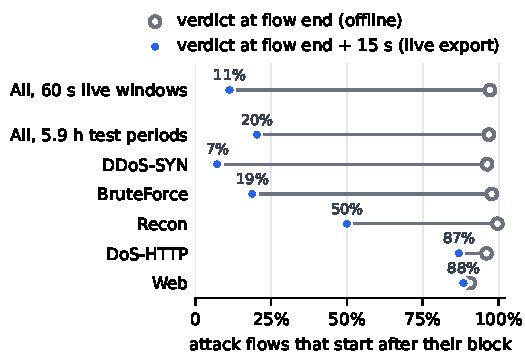
\includegraphics[width=\columnwidth]{late_blocks.pdf}
\caption{Share of attack flows that start after their host pair is blocked ($k=1$, MITM-ARP verdicts ignored), with each verdict stamped at flow end, as an offline evaluation does, or 15\,s later, when the live gateway exports the flow (idle timeout). Top: pooled over run~1's ten 60\,s windows, counters reset per window (logged live verdict times: 11.1\%). Below: the 5.9\,h test periods with persistent counters and corrected labels, pooled and per class (MITM-ARP and Mirai, 35 flows, omitted).}
\label{fig:lateblocks}
\end{figure}

\emph{Late blocks.} Offline policy scores overstate prevention (Fig.~\ref{fig:lateblocks}). On validation, over whole capture periods with each verdict stamped at flow end, 99.5\% of attack flows start after their pair is blocked. To separate window length from export delay, we replayed the rule on the same run-1 windows with three verdict times: at flow end, 97.1--97.2\% of attack flows start after their block (for $k\in\{1,3,10\}$); at flow end plus the 15\,s idle timeout, 11.3\%; at the logged live verdict time, 11.1\%. In these short windows the export delay, not the window cut, causes the drop: in the DDoS-SYN window the first verdict arrives 15.2\,s in, when 82\% of the attack flows have already started. Over the 5.9\,h test periods (persistent counters, $k=1$) the pooled share falls from 96.8\% to 20.3\%. The pooled value is dominated by the trimmed DDoS-SYN capture, which holds most attack flows in a 23\,s test period, but a long test period does not by itself protect a class: the loss ranges from small (DoS-HTTP 96\% to 87\%, web 91\% to 88\%) to large (port scan 99.6\% to 50\%; brute force, over 79\,min, 98\% to 19\%). Blocks still cut the later packets of long attack flows (34--71\% of the DDoS-SYN and DoS-HTTP windows' packets).

\section{Threats to Validity}\label{sec:threats}

\emph{Internal.} On CIC-IoT2023 the same author identified the attackers, wrote the labeling rule and made all design choices. The labels were revised once after error analysis (the sixth DDoS source), towards the model's predictions; a later blind audit in both directions found one more error, whose correction also favors the model (Benign FPR 1.3\% instead of 3.8\%; Section~\ref{sec:labels}). The audit's rater is a program, not a second person, and four of its rules were fixed after its first run (one a post-hoc criterion); we release its blind 975-flow sample for a manual check. Our CIC-IoT2023 results are scored against our own labels; IoT-23 supports the cost of file-name labels with the authors' labels but does not validate ours, and its file-name labels depend on our family mapping.

\emph{Construct.} Macro-F1 weighs tiny classes (Mirai, MITM-ARP) like large ones and, on IoT-23, missing classes; we report per-class results with host-pair counts. Without MITM-ARP, which flow features cannot see by the label's definition, macro-F1 is 0.826 instead of 0.725. False-block rates depend on the traffic mix and on the counting unit (60\,s host-pair windows live, host pairs over 5.9\,h in the replay), and the 60\,s reset hides some false blocks (Section~\ref{sec:response}).

\emph{External.} Labels and splits were audited on two datasets, but the live and response checks only on CIC-IoT2023, with one capture session per attack class, so they measure generalization within a session, not across networks. We do not test across datasets, where results are known to be asymmetric~\cite{ali2026siamxbert}. We audit one model: a random forest and gradient boosting score similarly on the temporal split (Section~\ref{sec:setup}), but we did not repeat the label and response checks with them. Large CIC-IoT2023 captures were trimmed, so a temporal split covers only their start. Live results hold only at the achieved replay rates, on one laptop under WSL2, and for floods that did not fill the capture buffer. Replay is open-loop, so ``packets dropped'' is counterfactual: drops cause no retransmissions, and attackers do not adapt.

\emph{Statistical conclusion.} The enforced settings ran once, and each pinned CPU budget three times. The SSH-to-RTSP change rests on three host pairs. Beyond it, the CIC-IoT2023 gap is small and not robust to the cluster unit (Fig.~\ref{fig:gapunits}). Per-class intervals over at most six host pairs are indicative only.

\section{Conclusion}\label{sec:conclusion}

Each check exposed a problem that the aggregate score of its stage could not show, from labels to blocking, and once in our own live results, where flow splitting left macro-F1 unchanged. We recommend that evaluations of flow-based NIDS (i) report each attack capture's background share and a leave-one-capture-out FPR; (ii) decompose a random--temporal gap per class and host pair, with class presence and the boundary-spanning share, before calling it drift; (iii) match live to offline flows one by one on every run, since an offline run flushes every flow at the end of the file; and (iv) score blocking in false blocks per host-pair window, with persistent counters and verdicts timed at flow export. Releasing CIC-IoT2023 flows with addresses and timestamps would let users relabel them. Future work includes a blocking criterion that weighs attack volume, not only flow verdicts, longer live runs, a second live dataset, early classification~\cite{pekar2025early} and edge hardware.

\subsection{Artifact Availability}

The repository \url{https://github.com/muhammadusamahoyrr/EdgeFlow-IDS} (MIT license) holds the code, attacker evidence, configuration, result files and audit scripts. The scripts recompute the offline numbers from the datasets; the live numbers also need the live flow logs, which are not in the repository. All random choices (split, trees, NSGA-II, bootstrap) use seed 0; live runs are timing-dependent. The NFStream fix is included (\nolinkurl{src/patch_nfstream.py}, diff in \nolinkurl{patches/}). The version used for this paper is the tag \texttt{v1.0-paper}.
% PLACEHOLDER for the author (do not compile in until minted): add the Zenodo DOI of tag
% v1.0-paper, e.g. "..., archived at Zenodo (DOI <to be minted>)".
The CIC-IoT2023 and IoT-23 data are available from their authors~\cite{neto2023ciciot2023,garcia2020iot23}.


\section*{Declaration of Generative AI and AI-Assisted Technologies in the Manuscript Preparation Process}
During the preparation of this work the authors used Anthropic Claude in order to help write the
experiment code and to draft and edit the text. After using this tool, the authors reviewed and
edited the content as needed; the first author directed the work and checked the experiments and
their outputs. Both authors take full responsibility for the content of the published article.

\bibliographystyle{IEEEtran}
\bibliography{refs}

\end{document}
